\documentclass[TechnicalNoteMeteo.tex]{subfiles}

\begin{document}

The algorithm described in this paper is based on the implementation of the classical MLR (Multiple Linear Regression) method presented in \cite{eischeid_creating_2000}. The MLR method is a robust and well known spatial interpolation technique that can indirectly account for local effects, such as topography, land cover, land use and surface water. While creating serially complete daily datasets of air temperature and total precipitation for the western U.S., \cite{eischeid_creating_2000} found that the MLR method consistently outperformed the other classical methods tested (normal ratio, inverse distance, optimal interpolation, and single best estimator). The same result was also found by \cite{xia_forest_1999} for a study in Bavaria, Germany. Moreover, in a study conducted in Iran for different climate conditions (dry to extra humid conditions), \cite{kashani_evaluation_2011} found that the estimation obtained with the MLR method compared well with those obtained with more recent methods, more specifically the artificial neural network (reference) and the genetic programming (references) techniques.

\Cref{fig:fillworker_flowchart} shows a flowchart of the gap-filling algorithm presented in this paper. The algorithm consists of two nested loops: the external `Loop A' iterates over the weather variables contained in the dataset of the target station (min, max, and mean air temperature and total precipitation), while the inner `Loop B' iterates over the missing values in the data series of the current weather variable in `Loop A'. Each missing value is estimated independently with a two-step procedure in `Loop B': the first step consists in the selection of the neighboring stations, while the second step consists in building a MLR model, estimating the missing value, and filling the corresponding gap in the data series. %Each step of the flowchart presented in figure X is dexribed in the following sections of this paper.

\begin{figure}[!p]
    \centering
    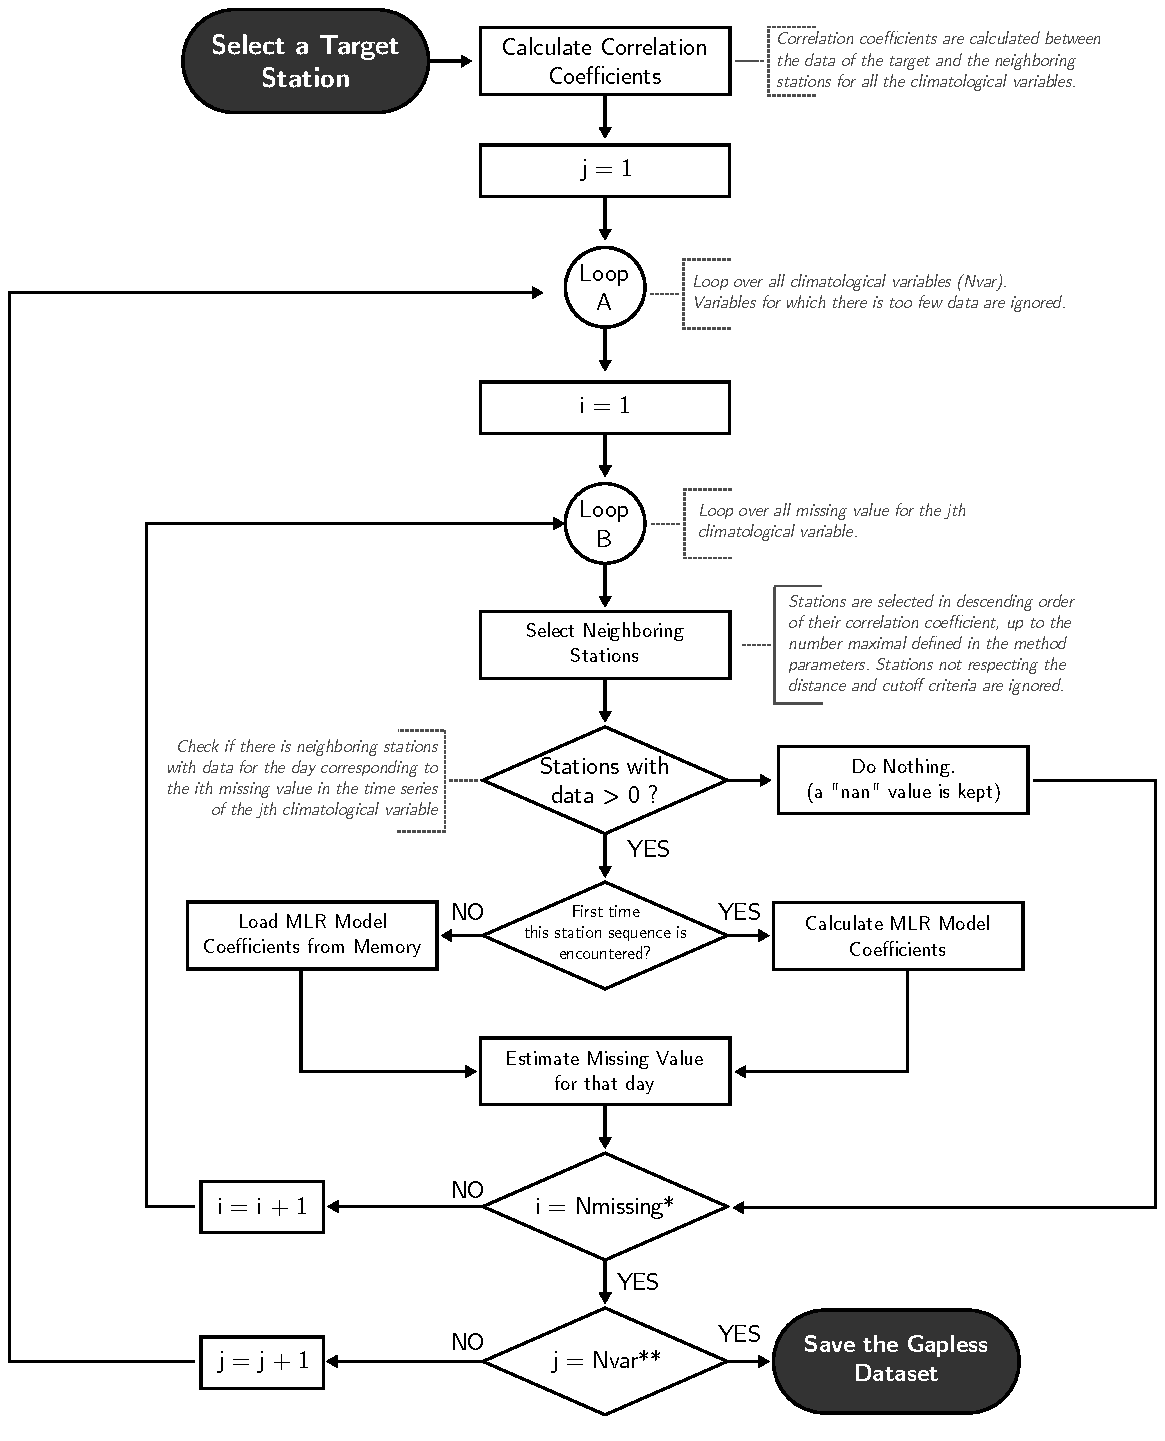
\includegraphics[width=\textwidth]{img/Flowchart-filling_missing_weather.pdf} 
    \caption{}
    \label{fig:fillworker_flowchart}
\end{figure}

\subsection{Correlation Coefficients Calculations}

Correlation coefficients are calculated between the available data of the target station and those of the neighboring stations for each weather variable individually, using all the available data. Neighboring stations that have less than 182 days (half a year) of synchronous data with the target station or that have a correlation coefficient below a value of 0.35 for a given weather variable are not used to fill the gaps in the data for that weather variable. The 0.35 threshold defined for the correlation coefficient is based on the value used by \cite{eischeid_creating_2000} in their application of the method. 

Moreover, it is possible to discard completely from the gap-filling procedure neighboring stations that are located further of the target station than specified thresholds, either in the horizontal or the vertical direction. The default values are set to \SI{100}{km} and \SI{350}{m} for the horizontal and vertical distance respectively, based on the values found in the literature \cite{tronci_comparison_1986,xia_forest_1999,simolo_improving_2010}.

\subsection{Selection of the Neighboring Stations}\label{sec:select_stations}

As stated by \cite{eischeid_creating_2000}, the selection of neighboring stations is critically important for the accurate estimation of missing weather data. Problems arise though because the list of neighboring stations with available data can vary from one day to the other. Therefore, the selection of the neighboring stations and the generation of a MLR model must be done individually for each day with a missing value in the dataset of the target stations.

Neighboring stations with available data are selected in descending order of their correlation coefficient, up the a maximal number of stations that is specified as a parameter of the algorithm. The default value for the maximal number of neighboring station used for the generation of the MLR models is 4. Tests run by \cite{eischeid_creating_2000} showed that using more then 4 neighboring stations did not significantly improve, and may even have degraded, the accuracy of the estimate. If for a given day with a missing value, no neighboring stations have a measured value, no calculation is done and a ‘NaN' value is kept in the dataset. 

\subsection{Generation of the Multiple Linear Regression Model}

Each time a MLR model is generated for a given sequence of neighboring stations, the resulting model parameters are stored into memory. Therefore, after the neighboring stations have been selected for a given day with a missing data (\cref{sec:select_stations}), the program checks if this sequence of selected stations has already been encountered before for the current weather variable. If so, the stored MLR parameters will be used directly to estimate the missing data for the current day. Otherwise, the model will generate a new MLR model and will store the results into memory. Since a MLR model is generated only one time for a given sequence of neighboring stations, the algorithm becomes faster with time.

The MLR model can be generated using either an Ordinary Least Square (OLS) or a Least Absolute Deviations (LAD) criteria. For the OLS criteria, the MLR model is obtained by solving the linear matrix equation $\mathbf{X}\mathbf{a} = \mathbf{Y}$ by computing the $N \times 1$ parameter vector $\mathbf{a}$ that minimizes the Euclidean L2-norm $\left\Vert \mathbf{Y}-\mathbf{X}\mathbf{a} \right\Vert_2$, where $\mathbf{Y}$ is a $M \times 1$ vector containing the M daily data of the target station and $\mathbf{X}$ is a $M \times N$ matrix containing the M synchronous daily data of the N selected neighboring stations. (REFERENCE: Numpy Documentation)

However, daily precipitation series are generally characterized by long-tailed, positively skewed, distributions. In this case, the generation of the MLR model using the more robust LAD method is a more appropriate approach that will yield more reliable results than using the OLS method as described above \cite{menke_geophysical_1989,eischeid_creating_2000}. Resolution of the MLR model with the LAD method is achieved in the gap-filling algorithm using an iterative reweighted least-squares method. The downside in using the LAD method compared to using the OLS is an increase in computation time by about a factor 10.

% TODO: The above paragraph needs to be revized. A more documented method must be used instead, or I need to better understand what I am doing with valid references.

%https://en.wikipedia.org/wiki/Iteratively_reweighted_least_squares

\subsection{Estimating Missing Daily Values}\label{sec:est_miss_values}

Once the parameters of the MLR model are known, the missing value for the corresponding day at time $t_i$ can be estimated as follows:
%
\begin{equation}
    Y_p\vert_{t_i} = a_0 + \sum_{k=1}^{N} a_k \cdot X_k(t_i)
\end{equation}
%
where $Y_p(t_i)$ is the value estimated at time $t_i$ for the $j_th$ weather variable in the dataset of the target station , $X_k(t_i)$ is the synchronous available data of the $k_th$ neighboring stations, $a_k$ are the regression coefficients, and $N$ is the total number of selected neighboring stations used for the regression.

When all the missing values in the dataset of target station have been estimated and filled, the resulting gapless time series are saved in a file with a `.out' extension. Moreover, detailed information about the estimated values are also saved in an accompanying `.log' file. The outputs of the gap-filling algorithm are discussed in more details in \cref{sec:output}.

\subsection{Uncertainty of the estimated values}

Each time a new MLR model is generated from a sequence of neighboring stations, an estimation of the accuracy of the model is made for the weather variable for which missing data are being estimated. This is done by first using the model to estimate the values for the days in the data series of the target station for which there exists a measured value. The accuracy of the MLR model is then approximated by computing a Root-Mean-Square Error (RMSE) between the estimated values and the respective measured values. The RMSE thus calculated is saved, along with the estimated value, in the `.log' file.

The algorithm also includes a cross-validation re-sampling procedure to estimate the accuracy of the method to fill the gaps in the dataset with a more rigorous approach. The procedure to enable this functionality in the algorithm is presented in \cref{sec:parameters}. The procedure consists in estimating a value for each day of the dataset of the target station, even for days for which data are not missing. In other words, when this option is enabled, the loop B in the flowchart of \cref{fig:fillworker_flowchart} will iterate over all the days of the dataset instead of only iterating over days with a missing data. Before estimating a value for a given day, the corresponding measured data in the dataset of the target station is temporarily discarded to avoid self-influence of this observation on the generation of the MLR model. Therefore, a new MLR model must also be generated for each day independently. Since model parameters cannot be recalled from previous models, the computation time of the gap filling procedure is significantly increased, especially if the least absolute deviation regression method is selected.

LOO, Leave One Out.

After a value has been estimated for a given day, the corresponding observed data is put back in the dataset of the selected station. When a value for every day of the dataset has thus been estimated, the estimated values are saved in a file with the extension `.err', along with the `.log' and `.out' files described in \cref{sec:est_miss_values}. The accuracy of the method can then be estimated by computing the RMSE between the estimated weather data and the respective non-missing observations in the original dataset of the selected station. Though costly in computation time, enabling this option can provide interesting insights on the performance of the procedure for the specific datasets used for a given project.

Moreover, the graphs that are presented in Section blabla are also produced upon the completion of the gap-filling routine for a given station blablabla.

\end{document}

%Essentially, the classifier is trained on a subset of the training data set, and tested on the remainder. This process is repeated systematically so that all the points in the training set are tested.

%Cross-validation is a way to predict the fit of a model to a hypothetical validation set when an explicit validation set is not available.

%Thus if we fit the model and compute the MSE on the training set, we will get an optimistically biased assessment of how well the model will fit an independent data set. This biased estimate is called the in-sample estimate of the fit, whereas the cross-validation estimate is an out-of-sample estimate.

%\subsubsection{Quality Control}

%the correlation between the data of the neighboring and target stations will generally decrease as the horizontal distance and elevation difference between them increase. Therefore,

%It is not possible to use a single MLR model to estimate the missing values in the dataset of the target station all at once.
 
%Prior to the analysis of weather time series, it is important to apply quality control constraints to ensure that the data do not violate obvious constraints associated with minimum, maximum, and average daily air temperature and daily cumulative precipitation. 

%The program will identify irregularities or inconsistencies to insure that maximum, minimum and average daily temperatures are coherent for a given day and that all daily precipitation values are positive. Erroneous values are replaced by nan values in the dataset. These values will subsequently be estimated by the program from neighboring stations.

%The first step of the procedure consists in the selection of the neighboring stations, whose data will be used to estimate the missing value in the dataset of the target station. The second step consists in building a MLR model and estimating the missing value.

%Among these techniques, methods based on the use of data from neighboring stations are generally favored to within-station methods, i.e. those that only use data from the series being filled.

%have been proven to perform poorly compared to methods based on the use of data from neighboring stations for the reconstruction of daily precipitation time series (Eischeid et al., 1995; Kemp et al., 1983; Simolo et al., 2010).

%The creation of a serially complete weather dataset generally consists in the replacement of missing daily data with estimated values calculated from simultaneous observations at nearby stations. 

%Numerous spatial interpolation techniques exist for handling the missing data in the weather time series of a given station by using data from irregularly spaced neighboring station (e.g. simple arithmetic averaging, inverse distance method, single best estimator and multiple regression analysis).

% An example of this problem is illustrated in \cref{tab:selectStations}, where theoretical time-series of air temperature data are presented. In this example, there are missing values in the dataset of the target station, Y, for days 2, 4, and 5. Therefore, the missing value on day 2 will be estimated with data from the neighboring stations X1, X3, and X4 since there is also a missing value on this day for station X2. All neighboring stations will be used for the estimation of the missing value on day 4. Finally, only stations X1 and X2 will be used for the estimation of the missing value on day 5.
%
%\begin{table}[!hb]
%\newcommand{\nan}{\multicolumn{1}{c}{\textbf{nan}}}
%\center
%\caption{This table shows some data}
%\begin{tabular}{
%S[table-format = 1]
%*5S[table-format = 2.1]
%}
%\toprule
%& {Target} & \multicolumn{4}{c}{Neighbors} \\
%\cmidrule(lr){3-6}
%{Day} & {Y} & {X1} & {X2} & {X3} & {X4} \\
%\midrule
%%\rowcolor{gray!30}
%1 & 11.0 & 12.0 & 12.0 & 12.5 & 10.0 \\
%2 & \nan & 12.0 & \nan & 13.0 & 12.2 \\
%3 &   7.5 &  8.5 &   8.5 &  8.0 &  8.9 \\
%4 & \nan &  6.0 &   4.5 &  5.0 &  4.4 \\
%5 & \nan &  8.0 &   8.5 & \nan & \nan \\
%\bottomrule
%\end{tabular}
%\label{tab:selectStations}
%\end{table}
